\section{Project Group}

In our project we are 13 students coming from 7 different countries.


\begin{table}
\centering
\begin{tabular}{|l|c|}
\hline
Group member & Nationality \\ \hline\hline
Jon Borglund & 
\includegraphics{graphics/se} \\
Paolo Boschini & 
\includegraphics{graphics/it} \\
Kiril Goguev & 
\includegraphics{graphics/bg} \\
Faroogh Hassan & 
\includegraphics{graphics/pk} \\
Marcus Ihlar & 
\includegraphics{graphics/se} \\
Alexander Lindholm & 
\includegraphics{graphics/se} \\
Knut Lorenzen & 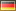
\includegraphics{graphics/de} \\
Harold Mart\'{i}nez & 
\includegraphics{graphics/ve} \\
Thomas Nordstr\"om & 
\includegraphics{graphics/se} \\
Thiago Costa Porto & 
\includegraphics{graphics/br} \\
Linus Sunde & 
\includegraphics{graphics/se} \\
Kim-Anh Tran & 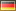
\includegraphics{graphics/de} \\
\hline
\end{tabular}
\caption{Each group member's nationality}\label{}
\end{table}

Due the scale of the project, the group decided to divide into two teams. 
The frontend team, responsible for implementing the client side of the NetInf project and the backend team, responsible for implementing the server technology.\\

The groups were divided as such:

The Frontend team(LISA)

\begin{itemize}
\item Kim-Anh Tran
\item Paolo Boschini
\item Harlold Martinez
\item Thiago Costa Porto
\end{itemize}

The Backend team(ERNI)

\begin {itemize}
\item Daniele Bacarella
\item Jon Borglund
\item Kiril Goguev
\item Faroogh Hassan
\item Alexander Lindholm
\item Knut Lorenzen
\item Thomas Nordstr\"om
\end {itemize}

\subsection{Seating arrangements}

The project rooms were divided into two areas, one room housing the frontend team aptly called LISA, the other housing the backend team aptly called ERNI. 